% File: algoritmo_1.tex
% Created: 2014-12-05
% Author: Tesser Paolo
% Email: p.tesser921@gmail.com
% 
%
% Modification History
% Version	Modifier Date	Author			Change
% ====================================================================
% 0.0.1	2014-12-05	Tesser Paolo		inserita sezione 
% ====================================================================
% 0.0.2	2014-12-06	Tesser Paolo		inizio stesura
%

\section{Algoritmo di risoluzione}
L'algoritmo scelto per risolvere il puzzle è di tipo sequenziale, come richiesto dalla specifica di progetto. \\
Per arrivare alla soluzione vengono utilizzati due strutture dati come membri della classe PuzzleCharacter. \\
La prima struttura è la collezione HashMap, nella quale vengono salvati in ordine casuale i tasselli ricevuti in input dal file di testo. Come chiave inserisco l'id del tassello mentre come valore uso l'intero pezzo (Tile). \\
La seconda struttura dati è un array bidimensionale di oggetti Tile. In essa andranno memorizzati i vari pezzi in ordine corretto, questo contenitore infatti rappresenterà il puzzle nell'ordine corretto alla fine dell'algoritmo. \\
Di seguito vengono esposte le sequenze che vengo eseguite, correlate da dei grafici che mostrano come esso agisca sulle strutture dati utilizzate.

	\begin{enumerate}
		\item \textbf{Ricerco il primo elemento del puzzle (quello in alto a sinistra).} \\
		Per fare ciò scorro una sola volta la tavola hash per cercare il tassello che ha id nord e id ovest uguale alla stringa VUOTO. \\
		Una volta trovato salvo il pezzo nella prima posizione dell'array bidimensionale.
		\begin{figure}[htbp]
			\centering
			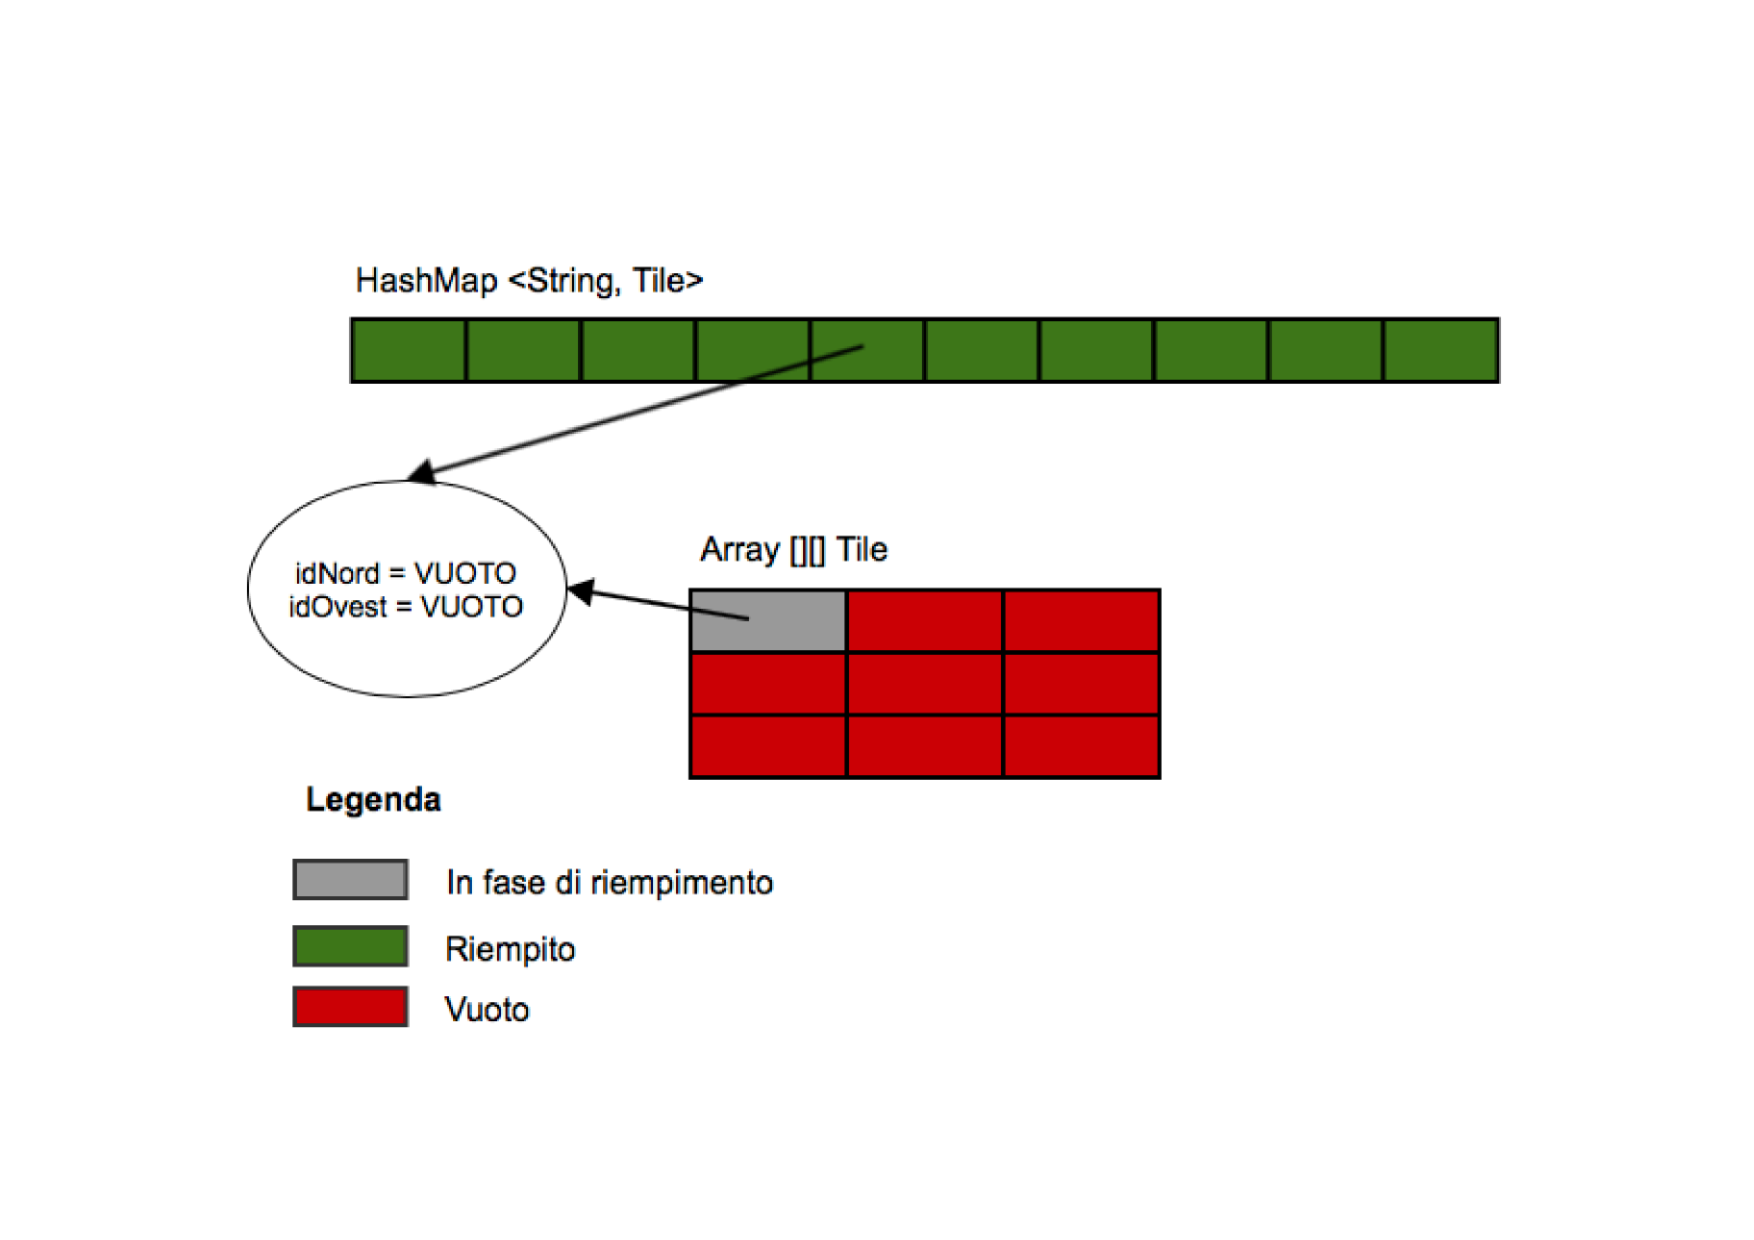
\includegraphics[width=15cm]{img/algpuzzle_step1.pdf}
			\caption{Algoritmo Step 1 - Ricerca del primo elemento}
			\label{Algoritmo Step 1 - Ricerca del primo elemento}
		\end{figure}
		
		\item \textbf{Ordino la colonna più a sinistra (quella con i tasselli aventi id ovest uguale alla stringa VUOTO).} \\
		Prendo l'elemento trovato al passo successivo, mi estraggo l'id sud di esso e tramite i metodi della tavola hash mi ricavo il tassello reale a cui corrisponde. \\
		Una volta estratto lo inserisco nella posizione corretta. \\
		Continuo così da quello appena trovato fino a quando non trovo tutti quelli sottostanti.
		\begin{figure}[htbp]
			\centering
			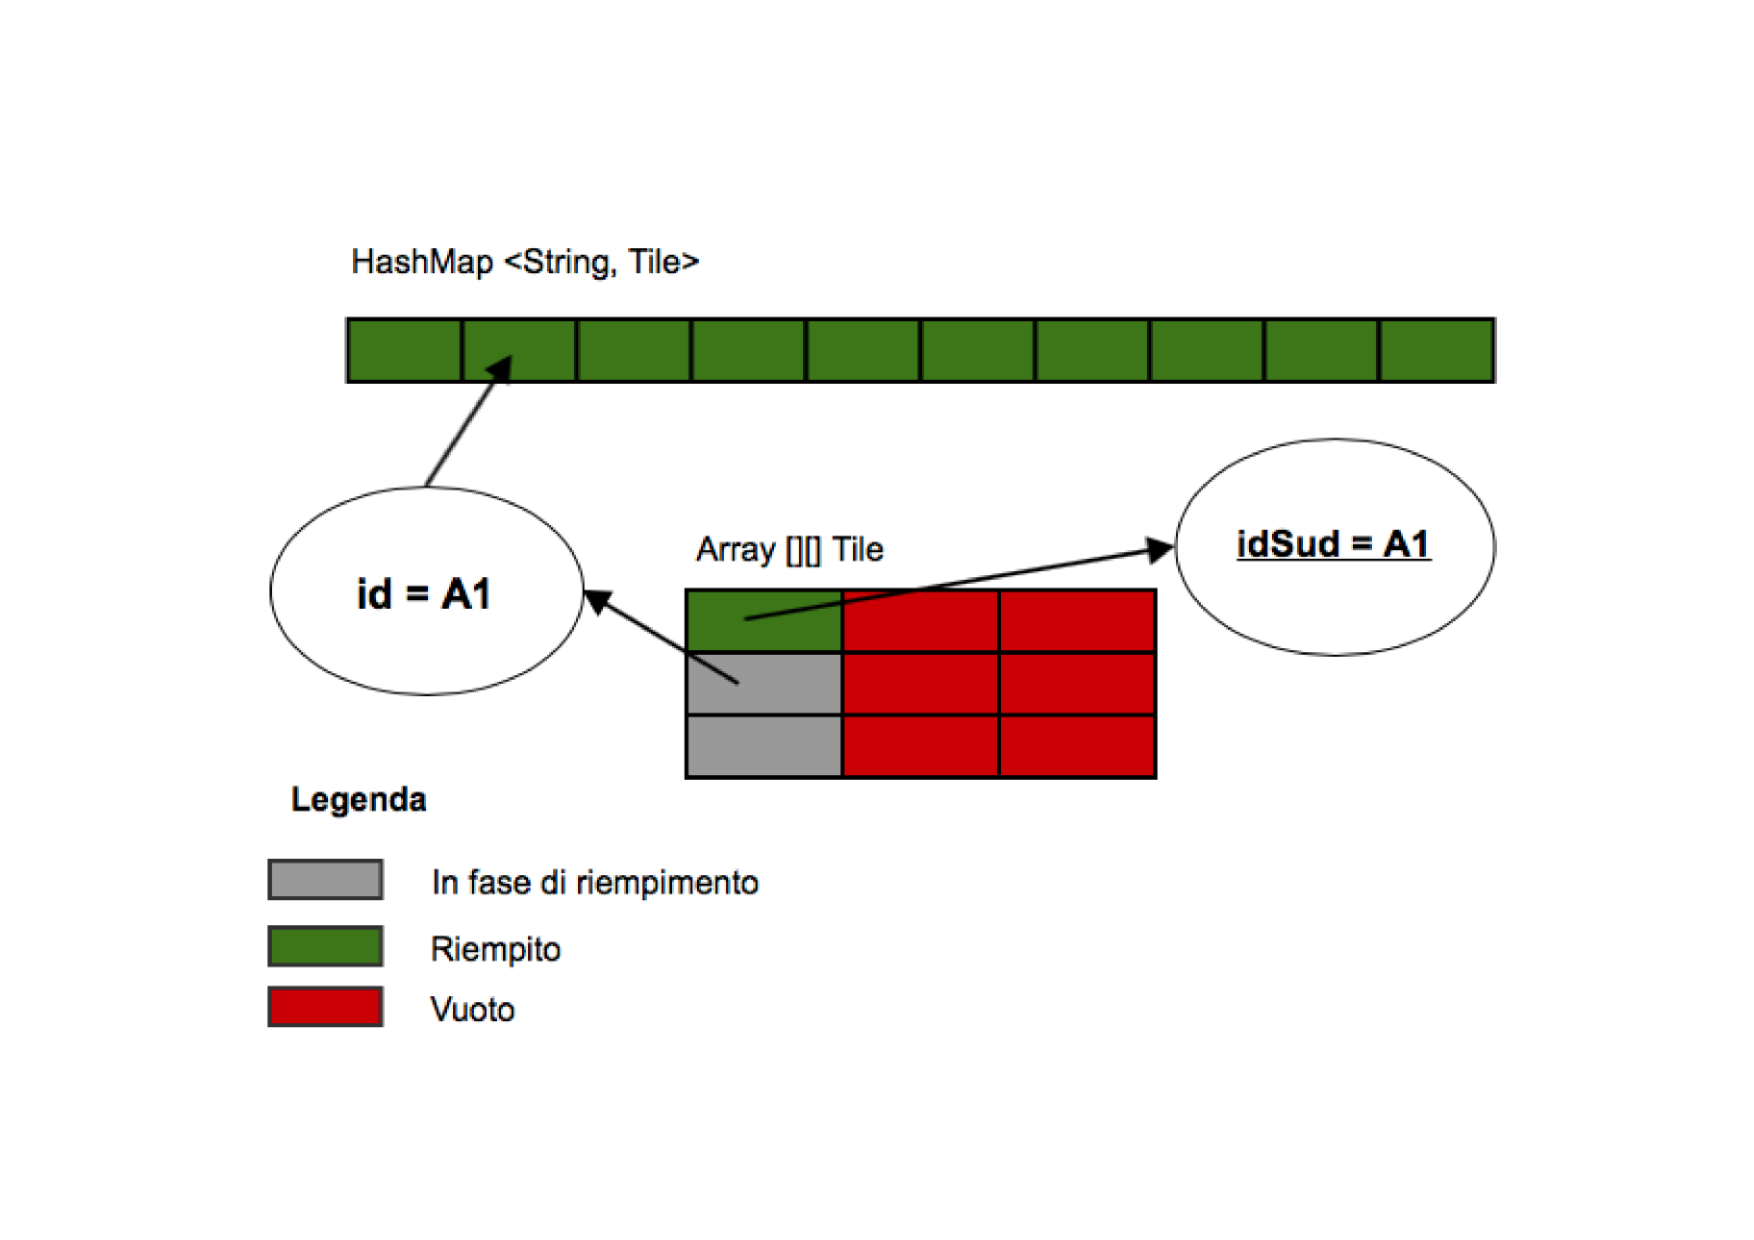
\includegraphics[width=15cm]{img/algpuzzle_step2.pdf}
			\caption{Algoritmo Step 2 - Ricerca della colonna più a sinistra}
			\label{Algoritmo Step 2 - Ricerca della colonna più a sinistra}
		\end{figure}

		\item \textbf{Ordino tutte le righe.} \\
		Dopo aver ricavato tutta la prima colonna, eseguo, secondo lo stesso principio, anche la risoluzione per le righe, procedendo però sta volta con la ricerca del pezzo successivo a destra tramite l'id est.
		\begin{figure}[htbp]
			\centering
			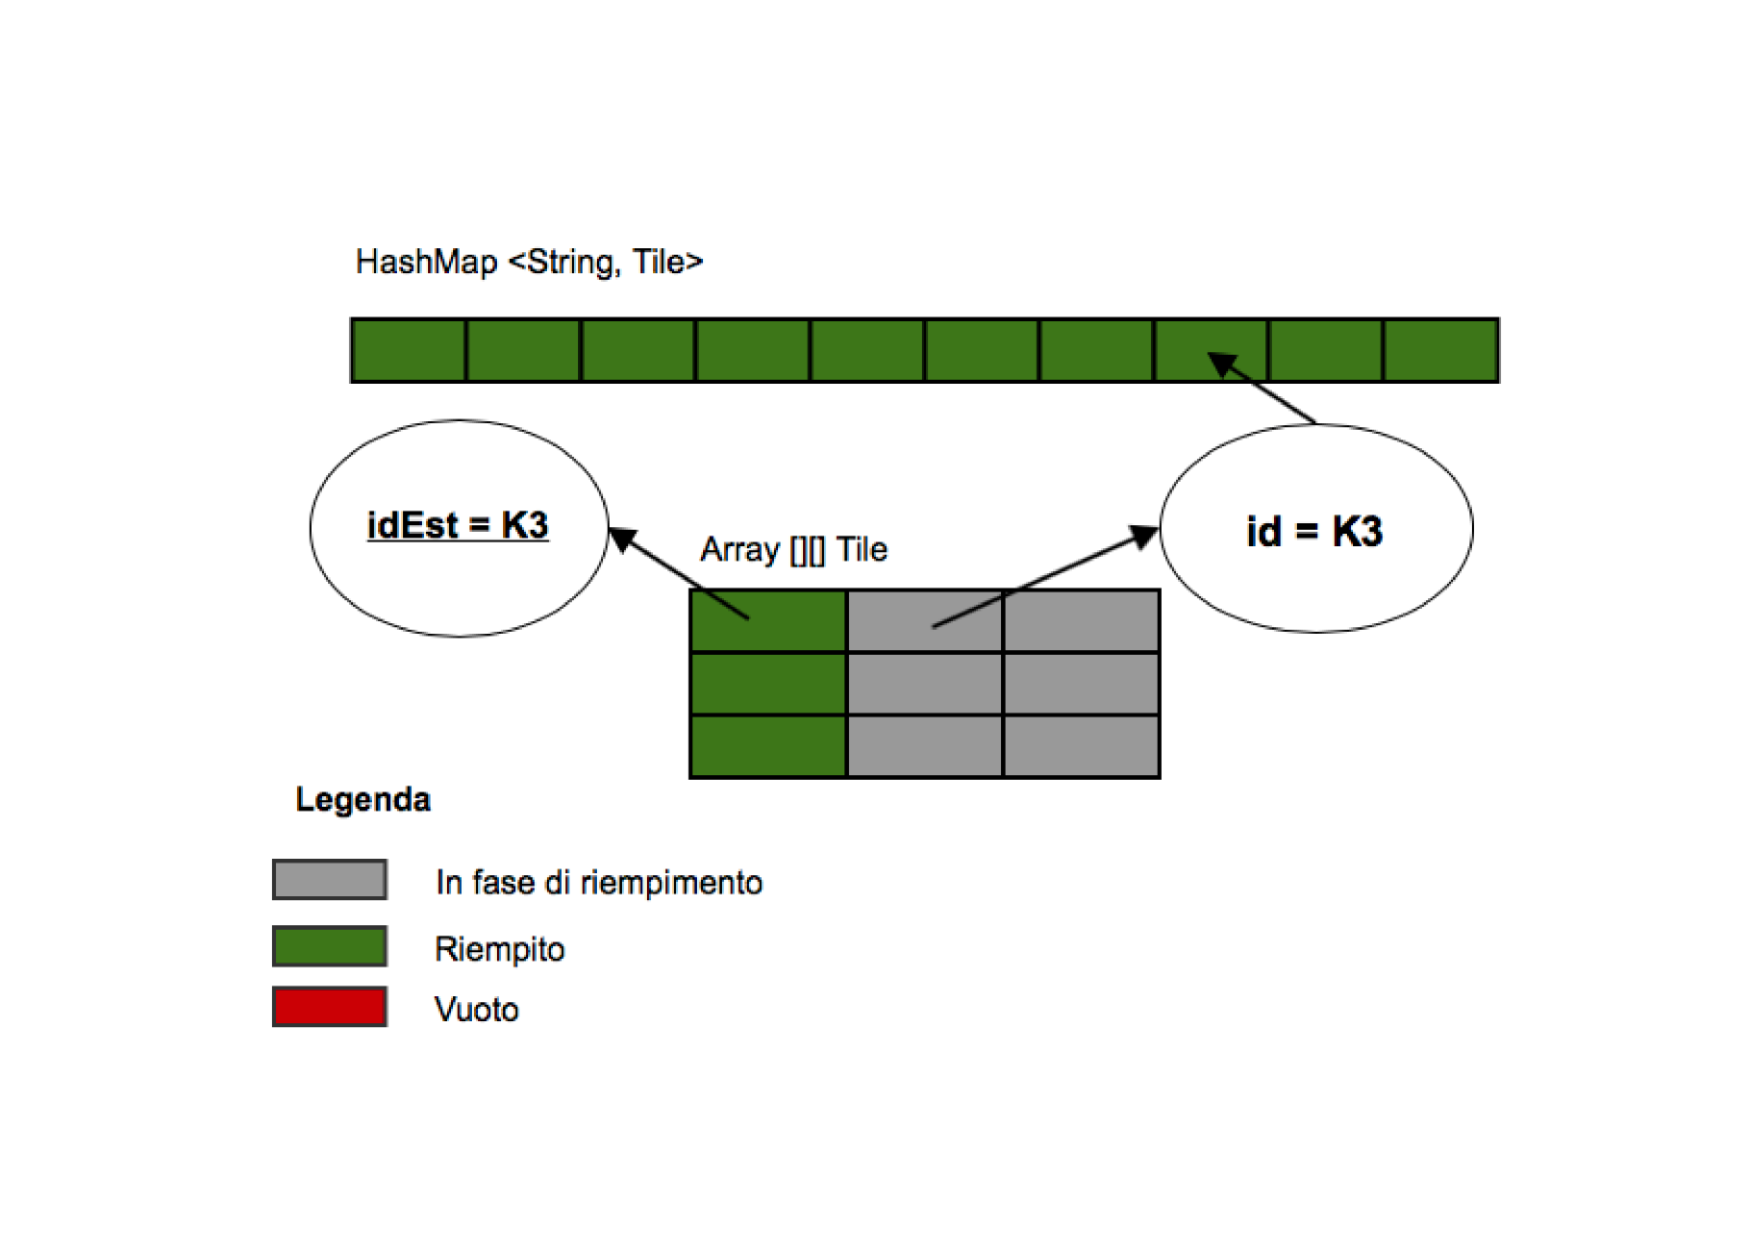
\includegraphics[width=15cm]{img/algpuzzle_step3.pdf}
			\caption{Algoritmo Step 3 - Ricerca delle righe}
			\label{Algoritmo Step 3 - Ricerca delle righe}
		\end{figure}

	\end{enumerate}


